\chapter[Mozart and Piano Sonata No. 10, K. 330]{Wolfgang Amadeus Mozart - Piano Sonata No. 10 in C major, K. 330 (1784)}
Wolfgang Amadeus (W.A.) Mozart (1756-1791) was a prolific composer during the Classical period (1730-1820) of music. Mozart was born in Salzburg, in the Holy Roman Empire, on January 27, 1756\autocite{Burkholder_Grout_Palisca_2014}. He was born into a talented musical family, and by age five showed a prodigal ability in performance, specifically on the keyboard and violin \autocite{Eisen_Sadie_2001}. Mozart started performing as a court musician in the Salzburg court when he was 17, and began traveling. These travels eventually brought him to Vienna in 1781, where he chose to stay. While in Vienna, Mozart composed his \textit{Piano Sonata No. 10 in C Major}. This sonata has three movements, the allegro moderato in C Major, the Andante cantabile in F Major\footnote{This movement is in C Major's subdominant key, an important concept explained later.}, and the allegretto movement. 

The \textit{Piano Sonata in C Major} follows the standard structure of a sonata. A sonata is known to be an instrumental piece which contains one or more movements, and designed to be performed by either a soloist or a small ensemble\autocite{Mangsen_Irving_Rink_Griffiths_2014}. Each period of music had its own specific definition of a sonata, and the Classical period was no different\footnote{As stated by Mangsen et al., the definition of a sonata evolved. The definition of a sonata started generally as an instrumental piece in the thirteenth century, and was known as a \say{sonnade.} Through the development of instrumental music in the following centuries, the current definition of a sonata comes from its connotations and associations in the Classical and Romantic periods of music. The sonatas of these times were frequently assumed to be instrumental pieces in which one or more movements are incorporated.}\autocite{Mangsen_Irving_Rink_Griffiths_2014}. Though definitions vary, generally the Classical period sonata is understood to be a musical work composed of three or four movements, most often for a piano solo \footnote{A duo between instruments such as the violin and piano were other popular choices.}. The first movement may be preceded by a slow introduction, but it is normally in sonata form. This is followed by a slow second movement, in which the key modulates to another, related key. Finally, the third movement follows as a finale, which wraps up the work.\autocite{Mangsen_Irving_Rink_Griffiths_2014} Sonata form itself is composed of three sections in a two-part tonal structure.\footnote{This two-part tonal structure is known as \say{binary form.} Binary form is defined as a musical structure which consists of two sections, of roughly equal duration\autocite{Sutcliffe_Tilmouth_2001}}. This is often notated as \textit{AB}, or \textit{A$A^`$}. The form itself is characterized by the clear move to another key, followed by another clear return to the tonic key. At the end of the \textit{A} section, there is a conclusive-sounding arrival on a contrasting key (which is often the dominant key) to signify the end of the \textit{A} section. The \textit{B} section's key will then modulate to the key that was referenced at the end of the \textit{A} section. At the end of the \textit{B} section, there is a matching conclusive arrival to what we saw at the end of the \textit{A} section, this time returning to the tonic key found in the \textit{A} section. Both the \textit{A} and \textit{B} sections may also be marked by a repeat sign, to be played through twice.\autocite{Sutcliffe_Tilmouth_2001}

Of the three movements of the sonata form, we divide them into two tonal parts. First, there is the \say{exposition} section, which is the first in the two-part tonal structure. The exposition, as the first section in both the sonata form and the two-part tonal structure, will contain the themes through which the rest of the movement and the piece are to be based on. The exposition will open in the piece's tonic key, and concludes in a new key. This new key is typically the dominant key of the exposition section's key if the piece is in a major key\autocite{Webster_2001}--which is a fifth interval away from the key in the exposition. With the exposition conclusively arriving in a new key, the piece moves to the \say{development} section. Once the development section arrives, we have moved into the second part of the two-part tonal structure. This part of the tonal structure includes both the development and recapitulation\autocite{Webster_2001}. The development section takes the thematic material that was presented in the exposition section, and manipulates it, moving both themes and key away from the exposition.\footnote{Some of these thematic manipulations include reshaping the material on a motivic level, on a harmonic level, or on a counterpoint level, or some combination of these levels.} The ending of the development section will lead into the \say{recapitulation} section. This recapitulation section is the final section of the sonata form, and is also a part of the second section of the two-part tonal structure. It signifies the return to the tonic key of the exposition section\autocite{Webster_2001}, and restates the thematic material from that first section.

\section{Movement I: Allegro moderato}
The first movement in Mozart's \textit{Piano Sonata in C Major} is the Allegro moderato. As is typical of sonatas, this first movement is light and energetic, evidenced by Mozart's choice to use cut-time (two-four time instead of the more widely used four-four time), and the thirty-second notes instead of sixteenth notes, like the notes circled in blue in Figure \ref{fig:mozart-first-movement-first-theme}\autocite{Henle_1977}. There are two main themes, or subjects, which alternate between legato and staccato. These subjects are placed over an energetic bass voice, comprised of flowing eighth and sixteenth notes.

\begin{figure}
    \centering
    \includegraphics[width=\textwidth]{figures/mozart-first-movement-first-theme.jpg}
    \caption{The first of two themes seen in Mozart's \textit{Piano Sonata in C Major}}
    \label{fig:mozart-first-movement-first-theme}
\end{figure}

\begin{figure}
    \centering
    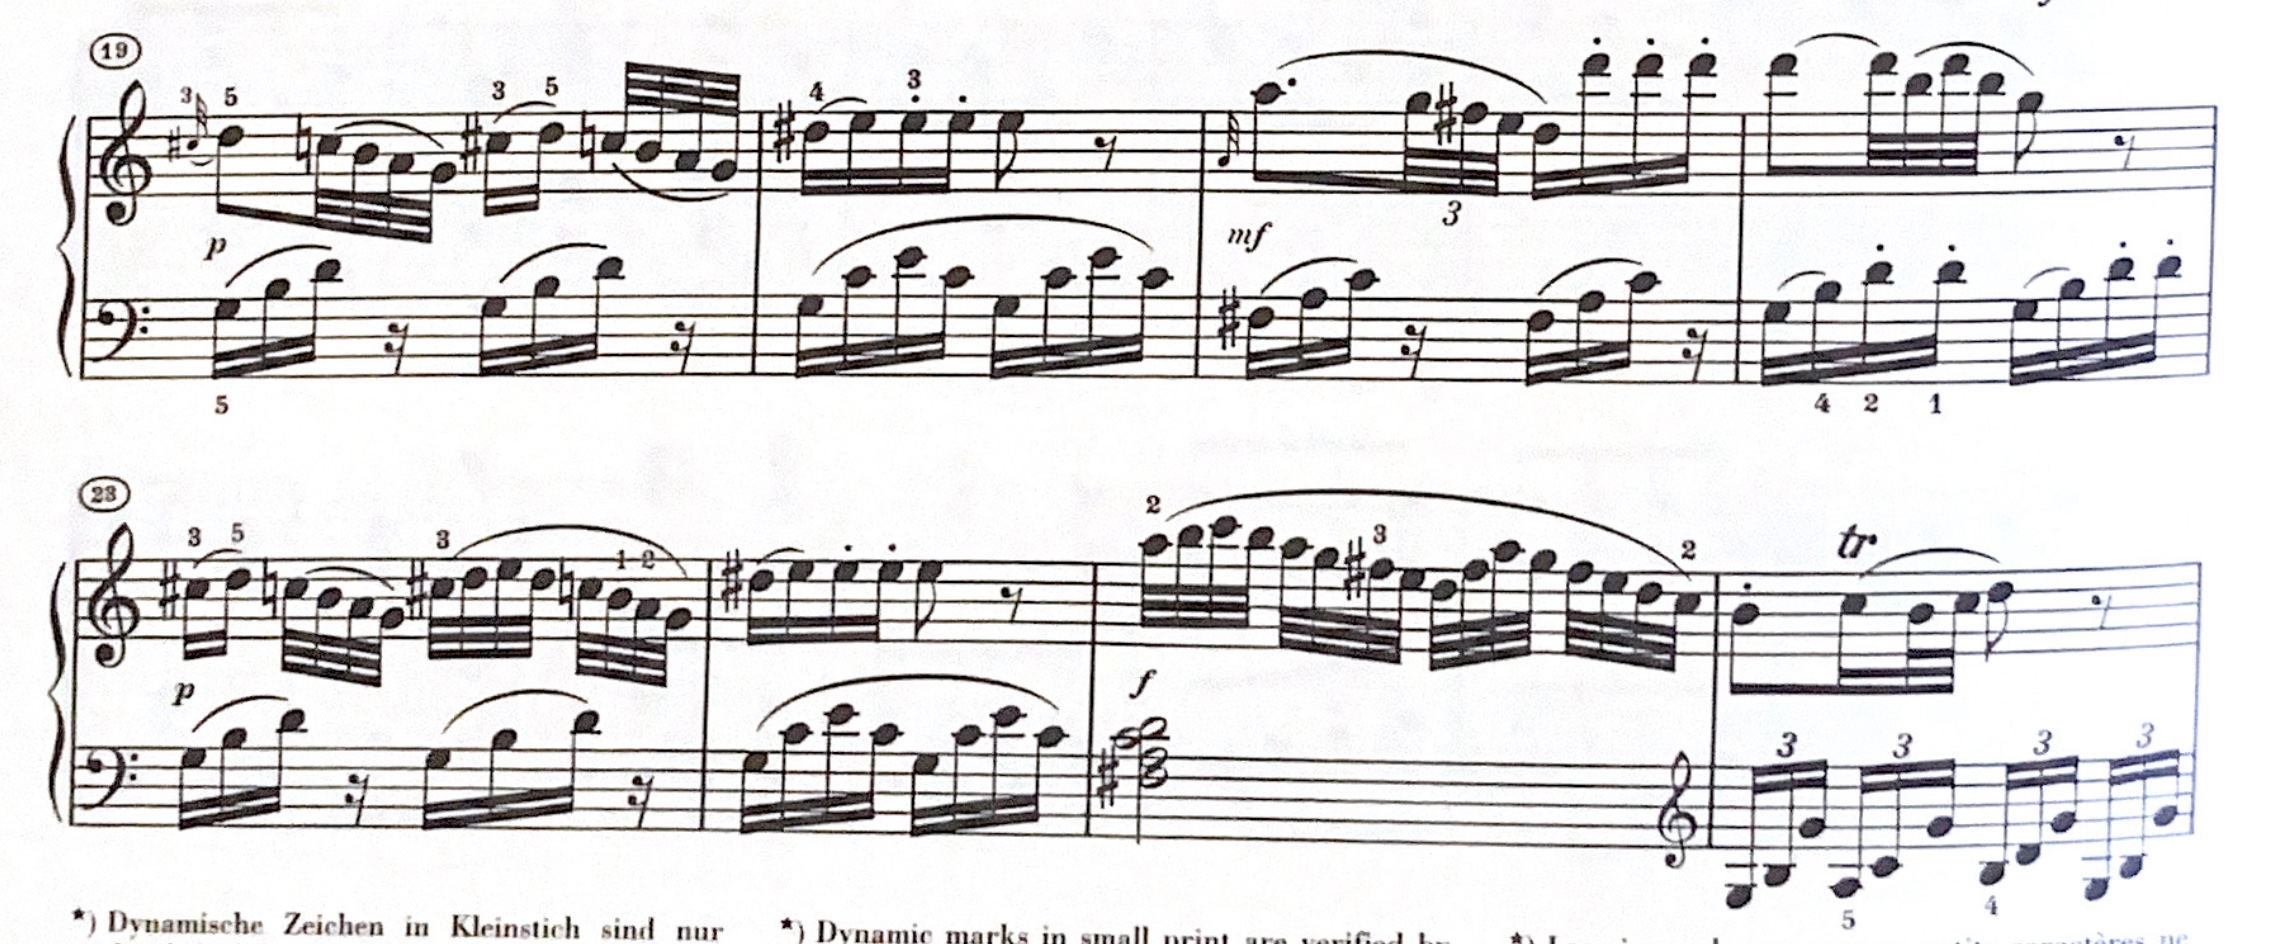
\includegraphics[width=\textwidth]{figures/mozart-first-movement-second-theme.jpg}
    \caption[The second theme in Mozart's \textit{Piano Sonata in C Major, K. 330}]{The beginning of the second of the two themes seen in Mozart's \textit{Piano Sonata in C Major}}
    \label{fig:mozart-first-movement-second-theme}
\end{figure}

The movement has two major themes, each decorated with ornamentation\footnote{This is defined as the decoration of a melodic or harmonic line in music.}\autocite{Latham_2011}\autocite{Burkholder_Grout_Palisca_2014}. The first twelve bars of the movement begin the exposition section. Within this section, we have two themes. The first theme, as seen in Figure \ref{fig:mozart-first-movement-first-theme}\autocite{Henle_1977}, lasts from bars one through twelve, and marked in red. This theme starts in the piece's tonic key of C Major. The second theme in Figure \ref{fig:mozart-first-movement-second-theme}\autocite{Henle_1977} begins in bar nineteen, and is marked by a modulation to G Major, the dominant key of the piece's tonic key C Major. The exposition section sets up the primary theme of the movement as a whole. The first theme, which is seen in Figure \ref{fig:mozart-first-movement-first-theme}\autocite{Henle_1977}, will be the theme through which the remainder of the movement is based on. The exposition's second theme, from Figure \ref{fig:mozart-first-movement-second-theme}\autocite{Henle_1977}, is also elaborated upon later in the piece. 

There is a development section introduced in bar fifty-nine, as in Figure \ref{fig:mozart-first-movement-second-theme}\autocite{Henle_1977}. This section is more intense than the exposition section, with more modulations. Bar sixty-nine and bar seventy show the modulation to A Major\footnote{See Figure \ref{fig:mozart-first-movement-modulation-a-major} \autocite{Henle_1977}}. This section also modulates to F Major, and D Minor\footnote{See Figure \ref{fig:mozart-first-movement-f-major-d-minor}}\autocite{Henle_1977}, before modulating back to the tonic key of C Major for the recapitulation section. In addition to the many modulations to related keys to the tonic C Major, the development section also contains references to thematic material of the first section. The bass voice in the first theme of the exposition section, as in Figure \ref{fig:mozart-first-movement-first-theme}\autocite{Henle_1977}, contains energetic sixteenth notes for the entirety of the theme. This is referred to in the development section, with bars fifty-nine to sixty-three, as in Figure \ref{fig:mozart-first-movement-development-reference-first-theme}\autocite{Henle_1977}, bracketed in red. 

\begin{figure}
    \centering
    \includegraphics[width=\textwidth]{figures/mozart-first-movement-development-reference-first-theme.jpg}
    \caption{The reference to the first theme in the exposition section, found in the development section, in Mozart's \textit{Piano Sonata in C Major}}
    \label{fig:mozart-first-movement-development-reference-first-theme}
\end{figure}

\begin{figure}
    \centering
    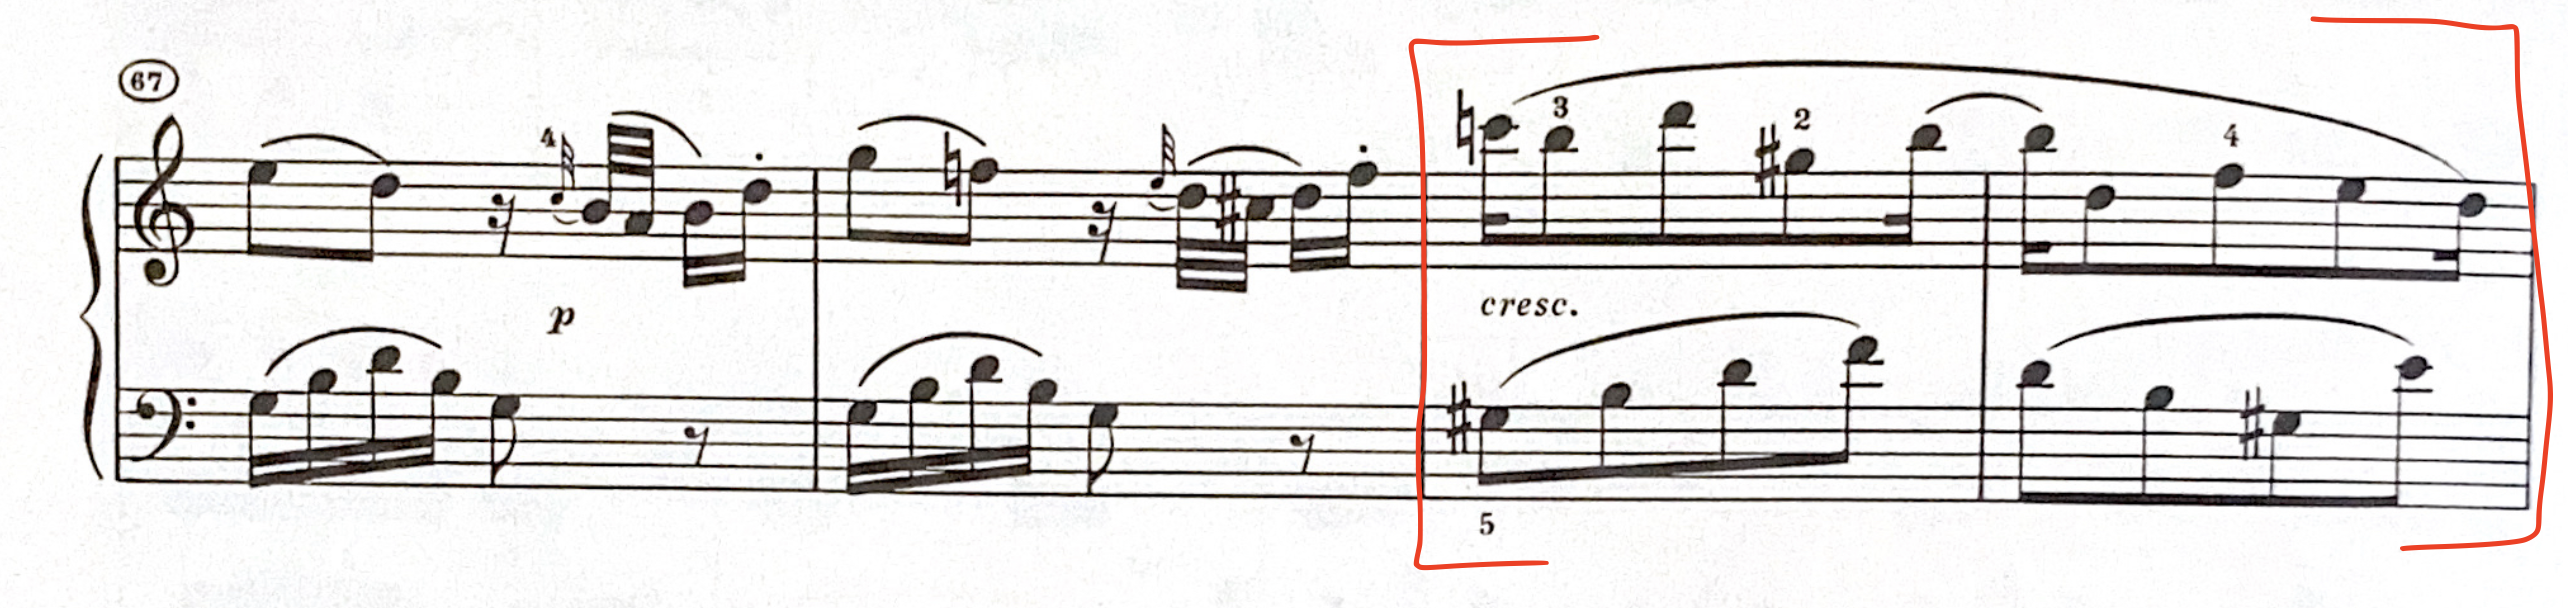
\includegraphics[width=0.5\textwidth]{figures/mozart-first-movement-modulation-a-major.jpg}
    \caption{The modulation to A Major, in Mozart's \textit{Piano Sonata in C Major}}
    \label{fig:mozart-first-movement-modulation-a-major}
\end{figure}

\begin{figure}
    \centering
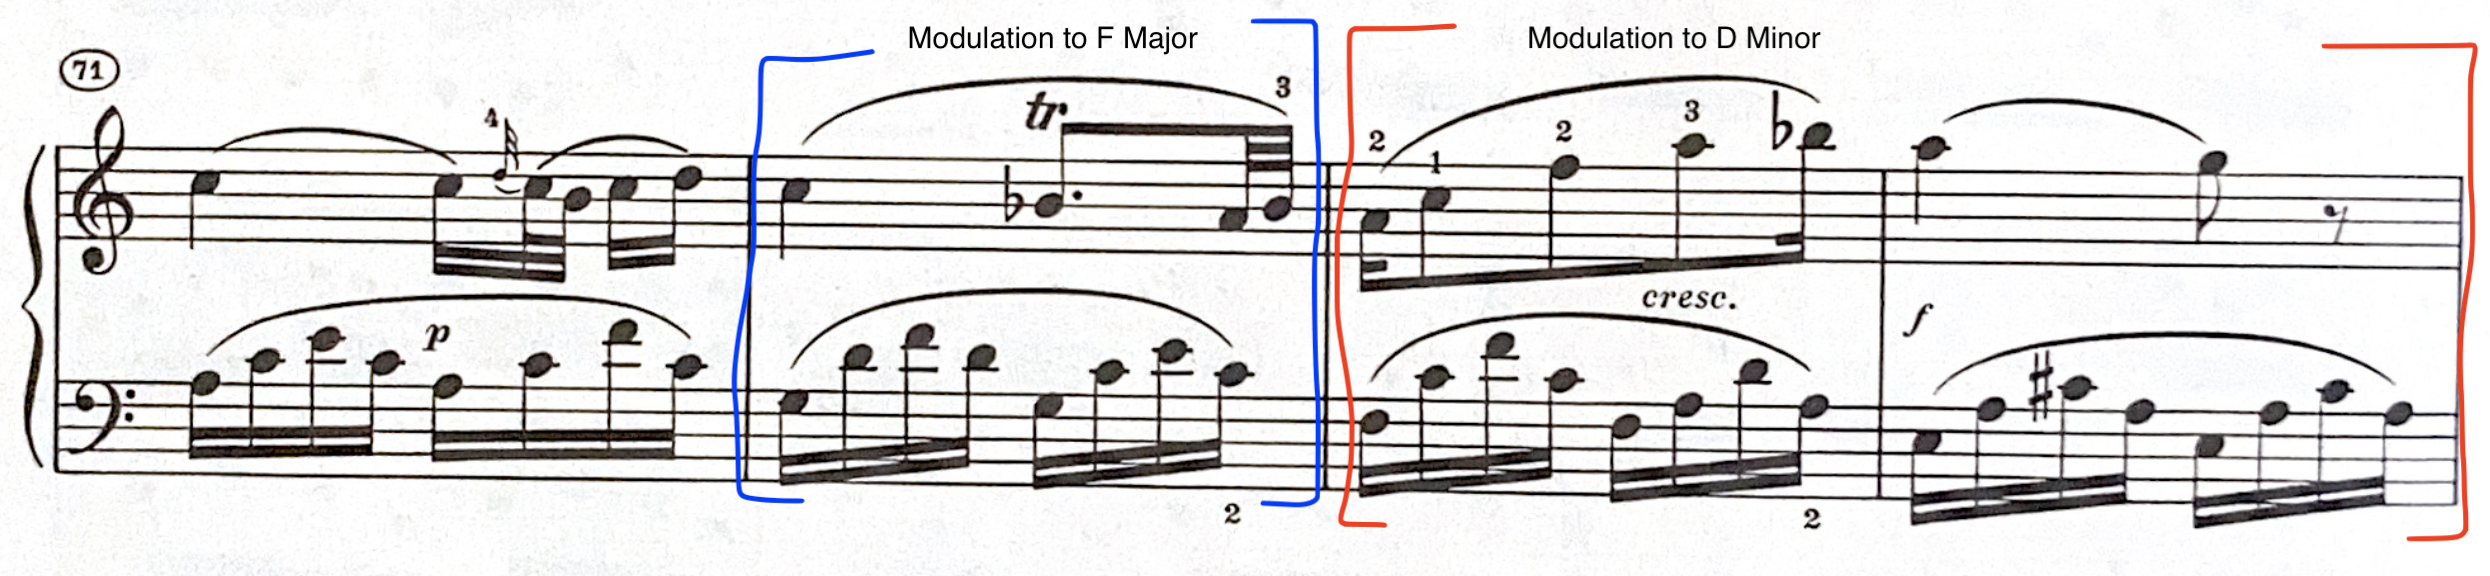
\includegraphics[width=0.5\textwidth]{figures/mozart-first-movement-f-major-d-minor.jpg}
    \caption{The modulation to D Minor, in Mozart's \textit{Piano Sonata in C Major}}
    \label{fig:mozart-first-movement-f-major-d-minor}
\end{figure}

\begin{figure}
    \centering
    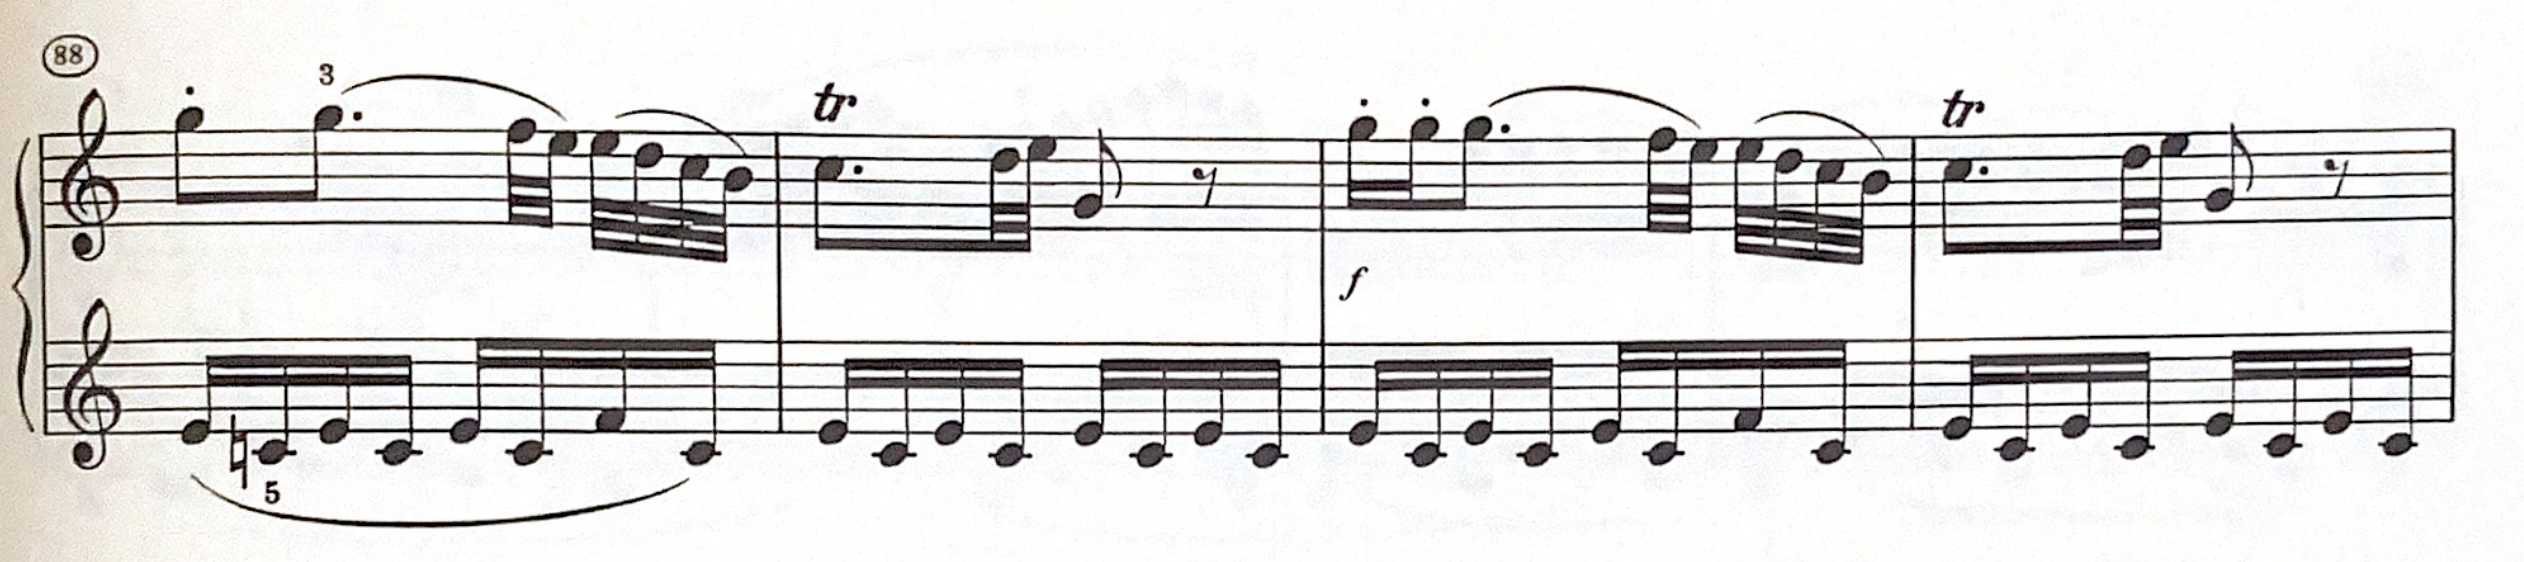
\includegraphics[width=\textwidth]{figures/mozart-first-movement-recapitulation-first-theme.jpg}
    \caption[The first theme of the exposition, found in the recapitulation, from Mozart's \textit{Piano Sonata in C Major, K. 330}]{The recapitulation section in Mozart's \textit{Piano Sonata in C Major}, where the first theme from the exposition section is heard again}
    \label{fig:mozart-first-movement-recapitulation-first-theme}
\end{figure}

Finally, in the recapitulation section, the first subject is heard again, in C Major, as in Figure \ref{fig:mozart-first-movement-recapitulation-first-theme}\autocite{Henle_1977}. The recapitulation section is similar in structure to the exposition section, with the first theme in tonic key C Major, and the second theme in dominant key G Major. There are few changes made to these two themes in this section, beyond a higher amount of ornamentation added to various bars. Thus, we see that the first movement itself is also in sonata form, with an exposition section, development section, and recapitulation section.

\section{Movement II: Andante cantabile}

\begin{figure}
    \centering
    \includegraphics[width=\textwidth]{figures/mozart-second-movement-first-a-section.jpg}
    \caption{The first A section of the second movement of Mozart's \textit{Piano Sonata in C Major}}
    \label{fig:mozart-second-movement-first-a-section}
\end{figure}

The second movement of Mozart's \textit{Piano Sonata in C Major}, the Andante cantabile, is marked with the modifier \say{cantabile,} meaning \say{song-like} and is reflected in the overall tonality of this movement being similar to a very sweet song. This movement is in ternary form\footnote{Ternary form is a musical structure which consists of three sections, hence the qualifier ternary. Its representation may be in the form of letter scheme ABA, with the final section A being a repetition of the first section. Each section of the ternary form is usually, but not always, self-contained and closes (or ends) in its key. The first A section will normally close in the tonic key. Then, the middle section will provide a strong contrast to the two sections which surround it, both in tone and theme.} and in the key F Major. This will be an important concept to note, as the first movement was in the tonic key of C Major. This movement modulates the key, from C Major to its subdominant F Major, and F Major's dominant key is C Major. The first \say{A} section, as bracketed in red in Figure \ref{fig:mozart-second-movement-first-a-section}\autocite{Henle_1977} can be broken into two parts. The first eight bars, as in Figure \ref{fig:mozart-second-movement-first-eight-bars}\autocite{Henle_1977}, begins this movement in the tonic key of F Major. With a few modulations to the dominant key of C Major, as in bars four through eight, the opening figure found in the pickup measure and first three bars is repeated and imitated several times. The four repeated C's are frequently used through this A section, and is repeated, both with the note C and the note G (bars four and five), leading to a repeated-note motif. This eight-measure figure is repeated with the repeat sign, before going into the twelve-bar sentence of the second part of the A section. 

The 12 bar sentence, as seen in Figure \ref{fig:mozart-second-movement-second-half-a-section}\autocite{Henle_1977} and bracketed in red, begins in the key of G Minor. One figure of note in this half of the A section is the similarity between bars seven and eight of the first half\footnote{For reference, in Figure \ref{fig:mozart-second-movement-first-eight-bars}.} of the A section, and bars 19-20 in the second half of the A section, or the last two bars as seen in Figure \ref{fig:mozart-second-movement-second-half-a-section}\autocite{Henle_1977}. There is a resemblance between how the first half of the A section ends (in bars seven and eight), and how the second half of the A section ends (in bars 19-20), which also ends the A section as a whole. The rhythms and figurations between these two sections are very similar, only with bars 19-20 modulated to a new key. This similarity between the endings of different parts is a notable feature of binary form\autocite{Sutcliffe_Tilmouth_2001}, which is used to indicate the two sections of a piece. This half of the A section also features other indicators of binary form, with key modulations to keys other than the dominant (G Minor, the minor second of F Major in bars nine and ten, B\musFlat{} Major in bars 14-16, the subdominant of F Major).

\begin{figure}
	\centering
	\includegraphics[width=\textwidth]{figures/mozart-second-movement-second-half-a-section.jpg}
	\caption{The second half of the A section, in the second movement of Mozart's \textit{Piano Sonata in C Major}}
	\label{fig:mozart-second-movement-second-half-a-section}
\end{figure}

\begin{figure}
	\centering
	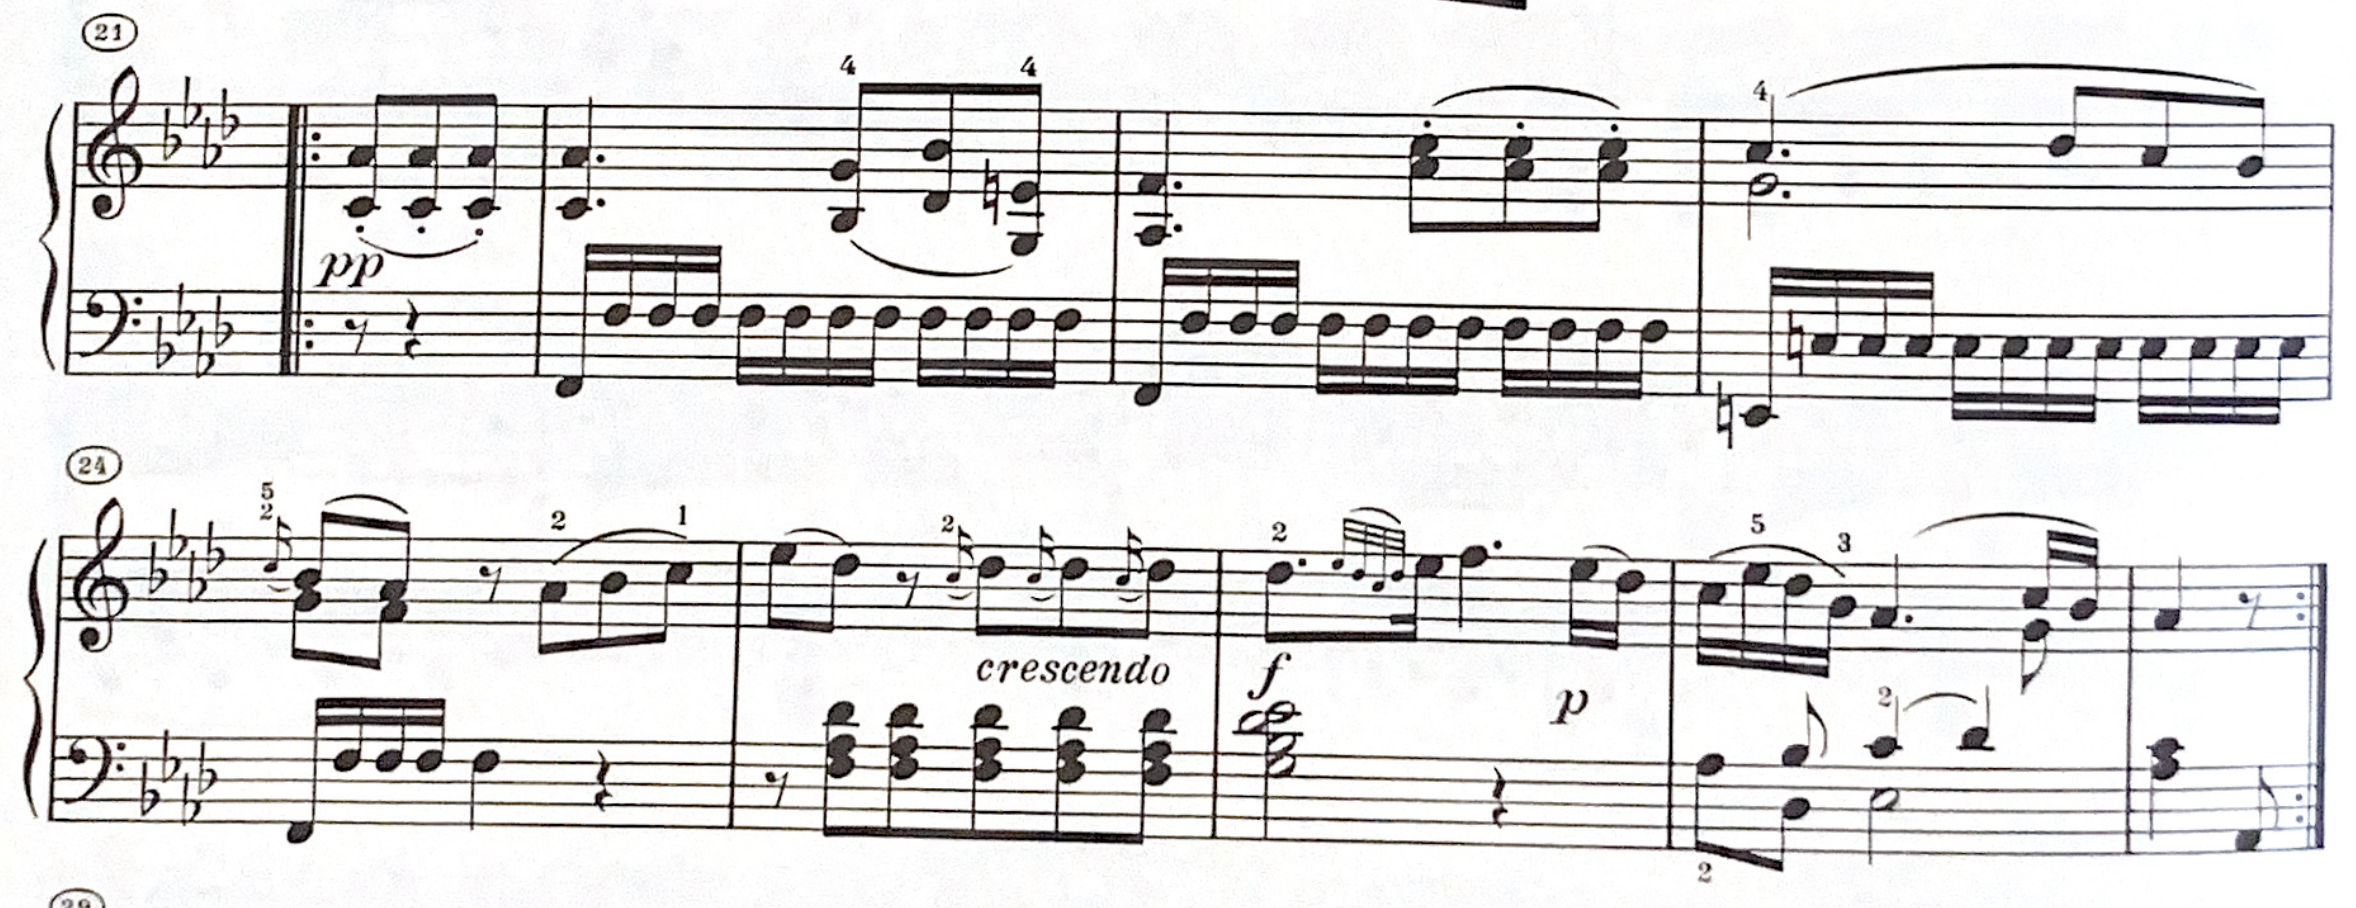
\includegraphics[width=\textwidth]{figures/mozart-second-movement-b-section-eight-bar-sentence.jpg}
	\caption{The eight-bar sentence, of the first eight measures in the second movement of Mozart's \textit{Piano Sonata in C Major}}
	\label{fig:mozart-second-movement-b-section-eight-bar-sentence}
\end{figure}

The B section of the second movement begins with an eight-bar sentence in the tonic key of F Minor. Much like the beginning of the A section, the eight-bar sentence here in the B section, as seen in Figure \ref{fig:mozart-second-movement-b-section-eight-bar-sentence}\autocite{Henle_1977}, is followed by a repeat sign, and contains a modulation. This sentence, in bar 23, modulates to the relative major key of A \musFlat{}. While not an uncommon modulation to make, it stands out in comparison to the A section's modulation to the subdominant key. After the repeat sign, the phrase continues in the key of A\musFlat{} Major. It is a transitionary phrase, in which the primary purpose of the phrase is to modulate back to the tonic key of F Minor. Then, the second part of the B section, bars 36-40, as seen in Figure \ref{fig:mozart-second-movement-second-half-b-section}\autocite{Henle_1977} and bracketed in red, is a restatement of the beginning of the B section. Bars 20-28\footnote{See Figure \ref{fig:mozart-second-movement-b-section-eight-bar-sentence} for reference.} contain the B section's original eight-bar sentence. In bars 36-40, there is a restatement of roughly bars 20-23. This is played over a pedal note\footnote{A repeated note in the left hand, to give the impression of one continuous note.} of the tonic note F. However, this eight-bar sentence is modified after the first phrase ends. It ends on a perfect cadence\autocite{Nagley_Whittall_2011} in the tonic key of F Minor\footnote{A cadence is known as a melodic or harmonic motion which is conventionally associated with the ending of a phrase, section, movement, or piece. This is a concept also discussed in chapter \ref{chapter:beethoven}.}. The perfect cadence\footnote{Other names for the perfect cadence include the final, full, or complete cadence, or the full close.} is a specific type of cadence in which a tonic chord is preceded by a dominant chord (either the chord a fifth above the tonic, or the chord a seventh above the tonic). The perfect cadence is considered to have the most finality of all the cadence types, and easily leads the listener to the next section of the piece.

\begin{figure}
	\centering
	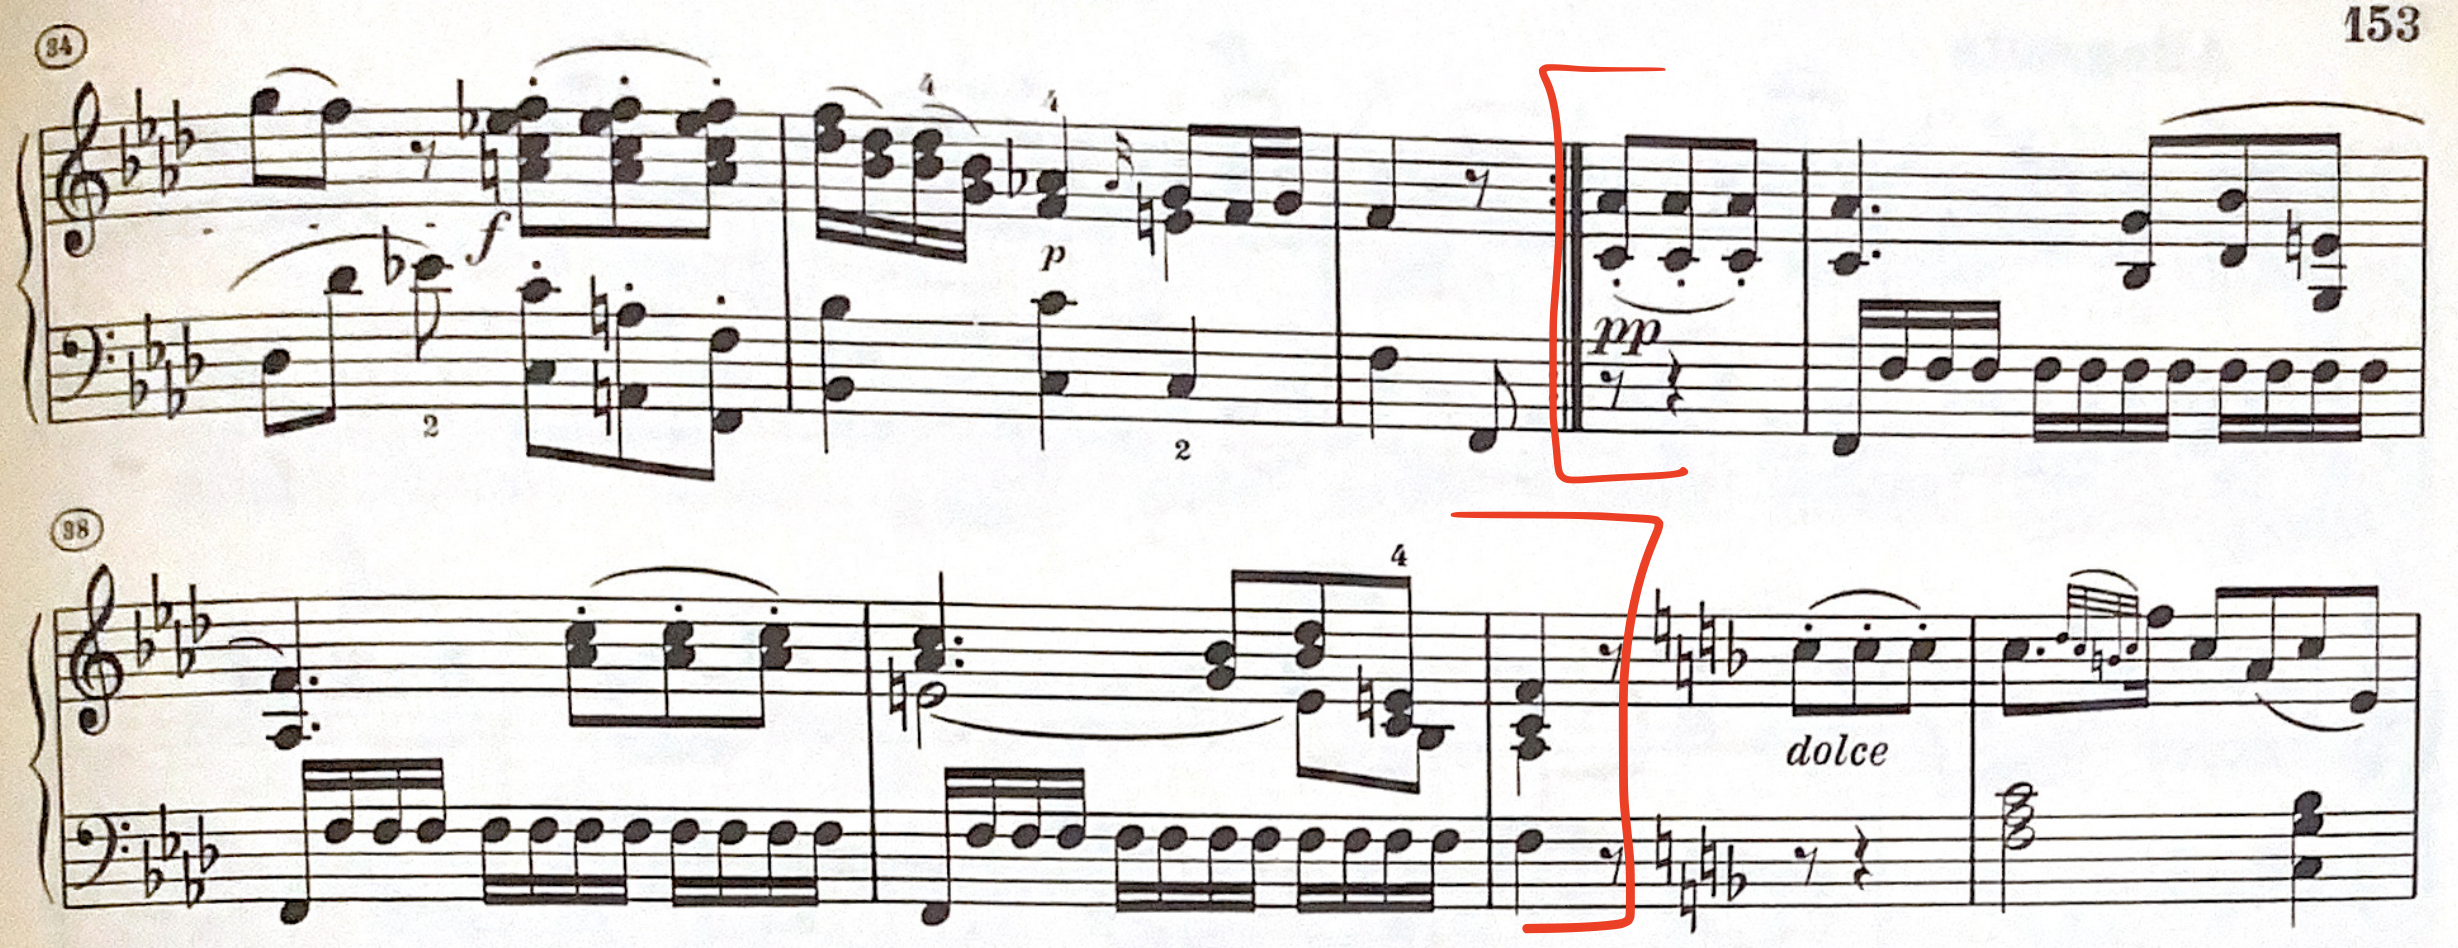
\includegraphics[width=\textwidth]{figures/mozart-second-movement-second-half-b-section.jpg}
	\caption{The second half of the B section, in Mozart's \textit{Piano Sonata in C Major}}
	\label{fig:mozart-second-movement-second-half-b-section}
\end{figure}

\begin{figure}
    \centering
    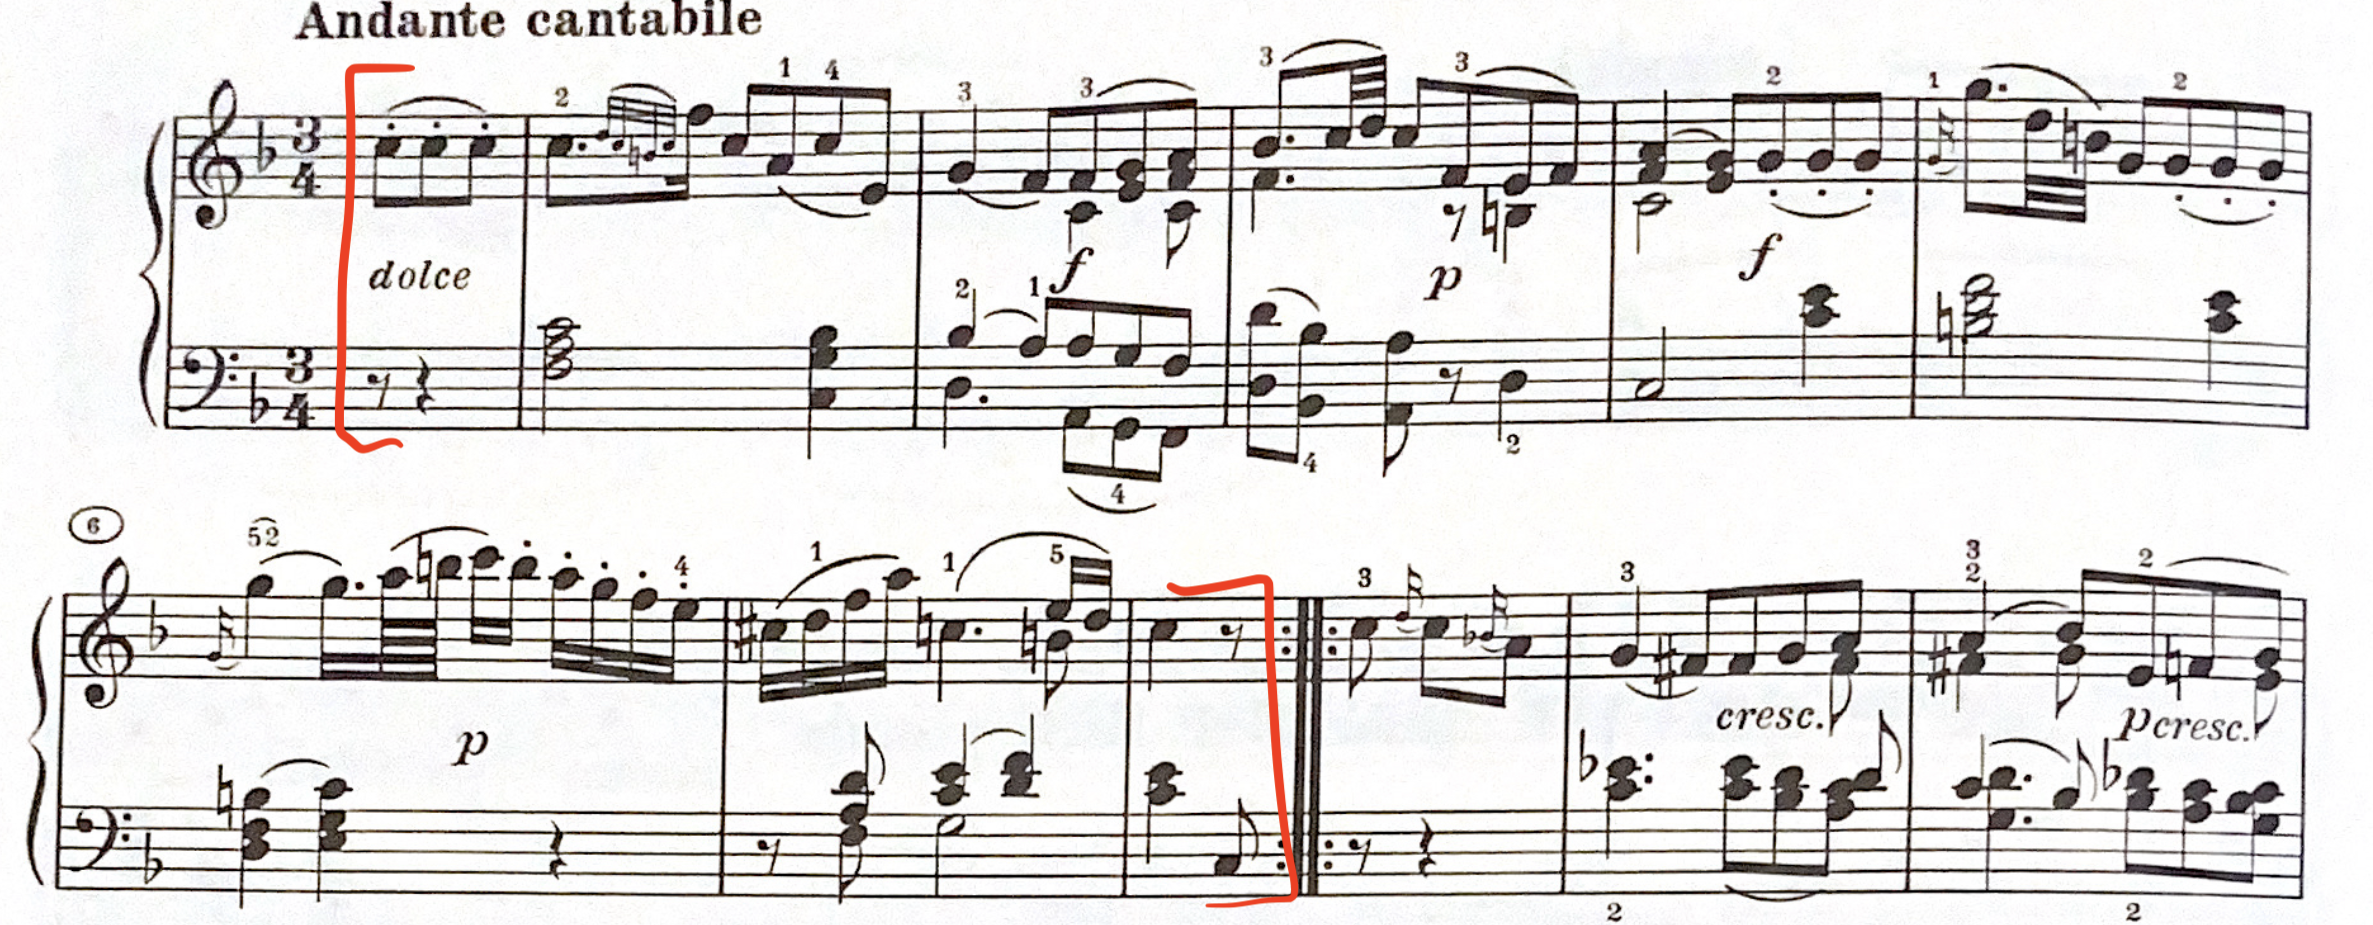
\includegraphics[width=0.5\textwidth]{figures/mozart-second-movement-first-eight-bars.jpg}
    \caption{The first eight bars of the second movement of Mozart's \textit{Piano Sonata in C Major}}
    \label{fig:mozart-second-movement-first-eight-bars}
\end{figure}

\begin{figure}
    \centering
    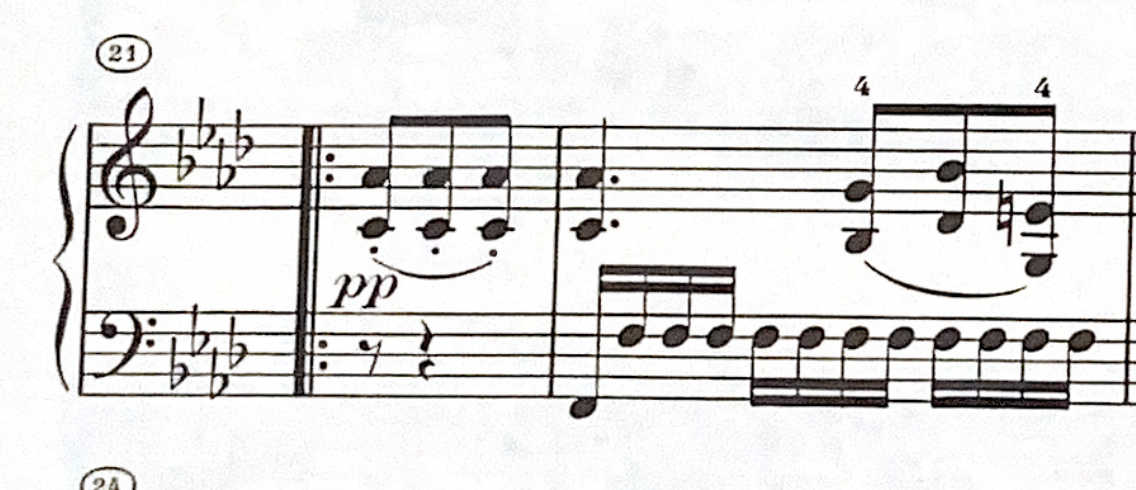
\includegraphics[width=0.5\textwidth]{figures/mozart-second-movement-repeated-note-motif-middle-section.jpg}
    \caption{The repeated-note motif, found in the middle section of Mozart's \textit{Piano Sonata in C Major} of the second movement}
    \label{fig:mozart-second-movement-middle-section-motif}
\end{figure}

\section{Movement III: Allegretto}
The third movement of Mozart's \textit{Piano Sonata in C Major} is the Allegretto, and is the piece's most energetic movement. Like in the first movement, this movement can also be classified as a sonata, as it is in sonata form. 

First, we have the exposition section, which introduces the thematic material which will be treated for the rest of the movement. The first 20 bars of the movement, as in Figure \ref{fig:mozart-third-movement-first-subject}\autocite{Henle_1977} and bracketed in red, introduce the first subject of the section. We are introduced to the subject in the tonic key of C Major again. The first sixteen bars comprise a long sentence. Beginning with bar one, there is an eight-measure phrase which is repeated with some variation in bars 9-16. With a perfect cadence in bar 16, between bars 17-20, there is a brief transitionary phrase in bars 21-32. At the end of the transitionary phrase, as in \ref{fig:mozart-third-movement-exposition-transition}\autocite{Henle_1977}, there is a modulation to G Major, the dominant key of C Major. The transitionary phrase ends on a half-cadence, indicating that the second subject for the exposition is next. The beginning of the second subject is in bar 33, as in Figure \ref{fig:mozart-third-movement-beginning-of-second-subject-exposition}\autocite{Henle_1977}. 

\begin{figure}
	\centering
	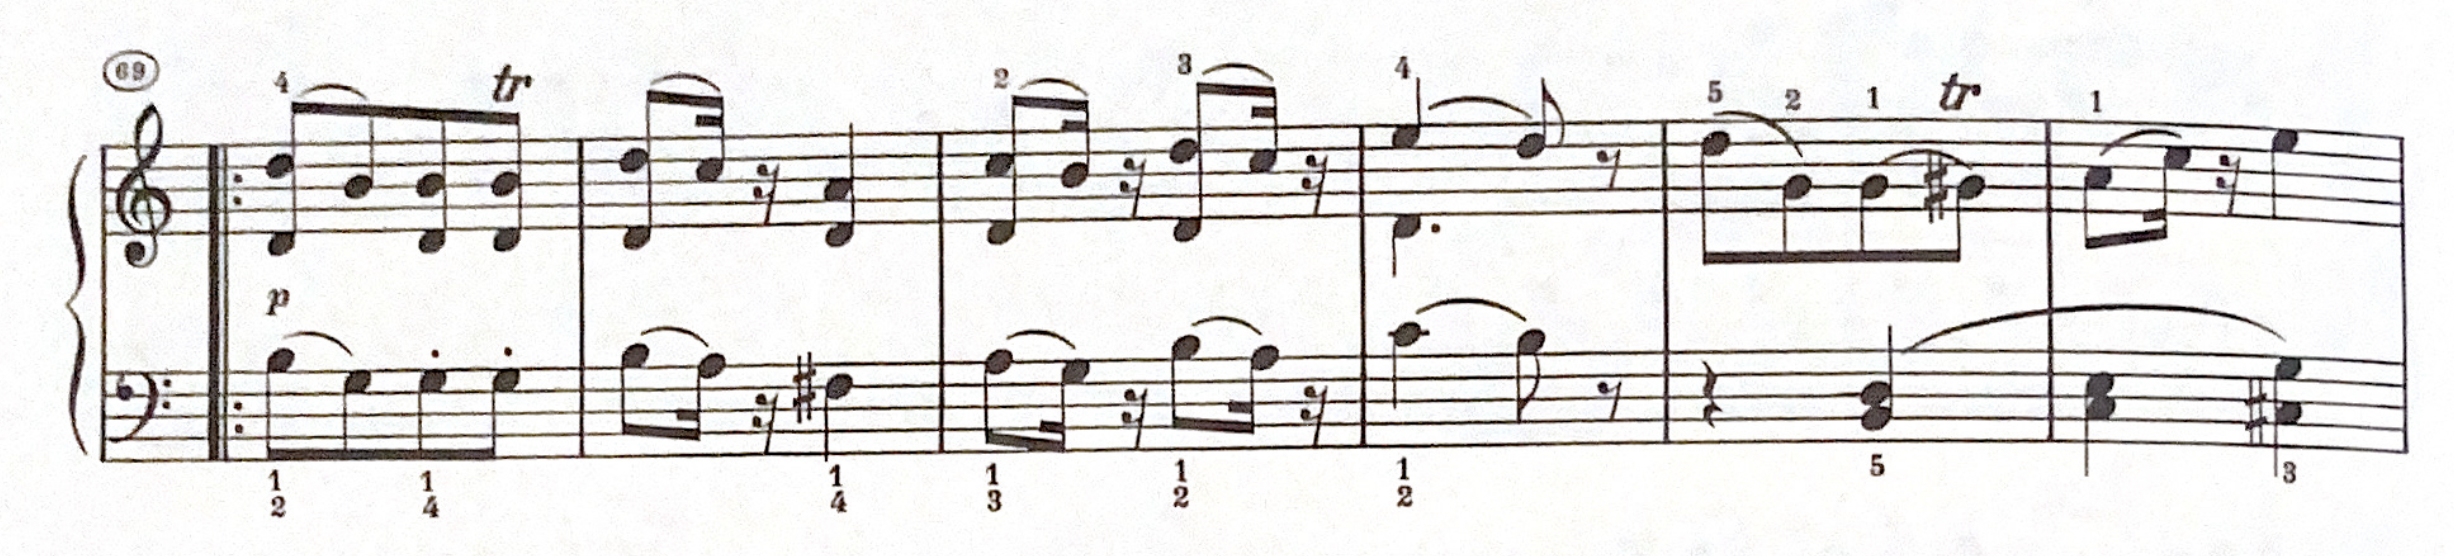
\includegraphics[width=\textwidth]{figures/mozart-third-movement-development-section-first-six-bars.jpg}
	\caption[The development section of Movement III, in Mozart's \textit{Piano Sonata in C Major}]{The beginning of the development section, in the third movement of Mozart's \textit{Piano Sonata in C Major}}
	\label{fig:mozart-third-movement-development-section-first-six-bars}
\end{figure}

\begin{figure}
	\centering
	\includegraphics[width=\textwidth]{figures/mozart-third-movement-bars-74-84.jpg}
	\caption{Bars 74-84 of the third movement in Mozart's \textit{Piano Sonata in C Major}}
	\label{fig:mozart-third-movement-bars-74-84}
\end{figure}

Then, there is the development section, which as seen in Figure \ref{fig:mozart-third-movement-first-subject}\autocite{Henle_1977} begins and contains no resemblance to the exposition section of the movement. The section as a whole is comprised of an episode\footnote{A type of phrase in which the subject of a passage is never fully stated in its entirety. There may be motifs throughout, however.}, with treatment of its own figures, rather than those in the exposition section. As this section works through its own figures, there is also treatment of the tonic G. Bars 77-83, in Figure \ref{fig:mozart-third-movement-bars-74-84}\autocite{Henle_1977} feature the frequent re-occurrence of tonic note G. Beyond this section's modulation into G Major from original tonic key C Major, there is no other modulation. Within this section, modulation is confined to the return to the tonic key (C Major) from the dominant key (G Major).

The return to the tonic key C Major indicates the beginning of the recapitulation section, and the third section of this movement's sonata form. Bars 96-115 repeat the structure found in this section's exposition section, as seen in Figure \ref{fig:mozart-third-movement-bars-96-107}\autocite{Henle_1977}. Bar 116, as in Figure \ref{fig:mozart-third-movement-bars-116-123}\autocite{Henle_1977}, then begins the section's transitionary phrase, connecting the recapitulation section's first subject and second subject. This transition passage is very similar to the transition section from the movement's exposition section, with some slight modifications and a lengthening of the section. As in Figure \ref{fig:mozart-third-movement-bars-124-129}\autocite{Henle_1977} and bracketed in red, bars 124-129 detail a typical modulation that happens in a sonata form's transition passage. This section is in the tonic key of C Major, and these bars feature a descending sequence as it modulates. First, the passage modulates to F Major, then to D Major, and finally back to tonic C Major. We receive a second subject between bars 132-160, and then are introduced to the movement's coda, as in Figure \ref{fig:mozart-third-movement-coda}\autocite{Henle_1977}. Between bars 160-171, we see that the coda is an extended repetition of the codetta found in the ending of the exposition section. However, unlike the original codetta, there is both a descending figure (bars 164-168) and then immediately after, there is a responding ascending figure. Full chords are also featured in the coda of this section, ending the movement on a sense of finality and a triumphant sound, typical of the sonata form.

\begin{figure}
	\centering
	\includegraphics[width=\textwidth]{figures/mozart-third-movement-first-subject.jpg}
	\caption{First subject of the third movement in Mozart's \textit{Piano Sonata in C Major}}
	\label{fig:mozart-third-movement-first-subject}
\end{figure}

\begin{figure}
	\centering
	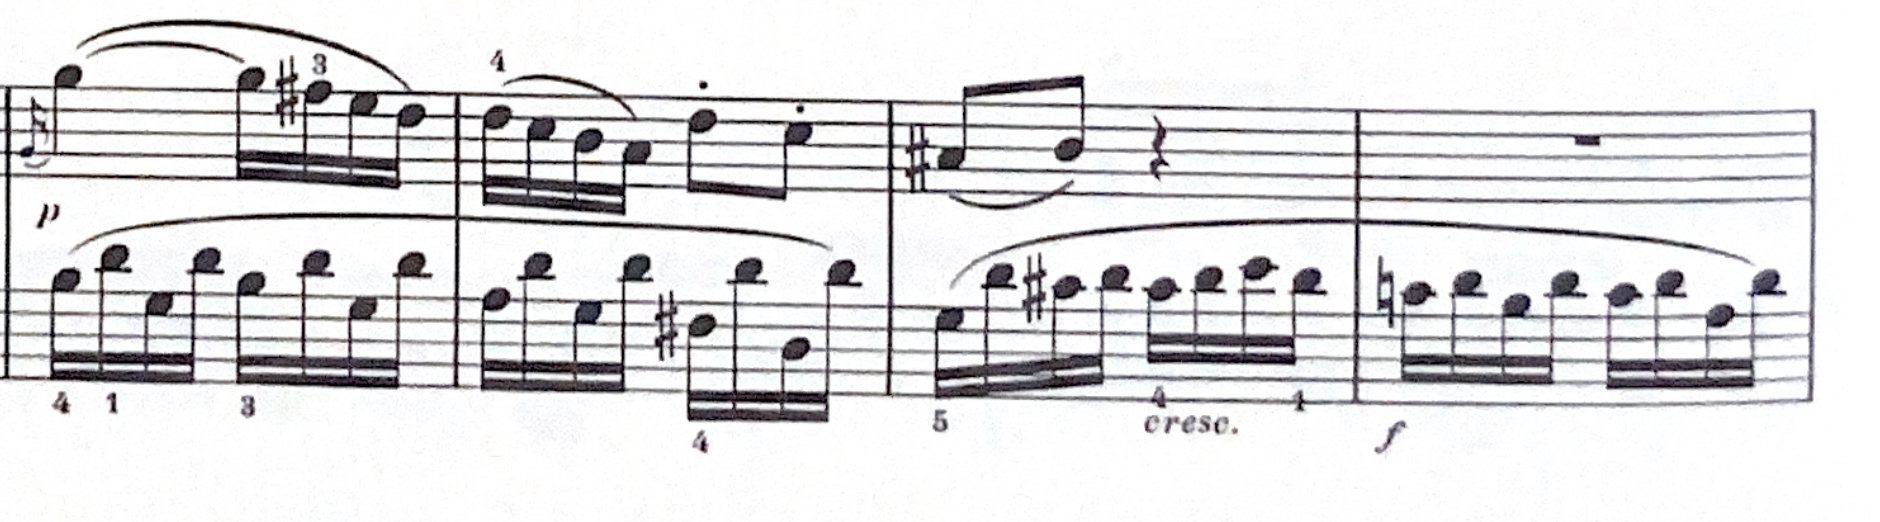
\includegraphics[width=\textwidth]{figures/mozart-third-movement-beginning-of-second-subject-exposition.jpg}
	\caption[Subject number two, in the third movement of Mozart's \textit{Piano Sonata in C Major}]{The beginning of the second subject, in the third movement of Mozart's \textit{Piano Sonata in C Major}}
	\label{fig:mozart-third-movement-beginning-of-second-subject-exposition}
\end{figure}



\begin{figure}
  	\centering
  	\includegraphics[width=\textwidth]{figures/mozart-third-movement-exposition-transition.jpg}
  	\caption{The transition section within the exposition, of the third movement, in Mozart's \textit{Piano Sonata in C Major}}
  	\label{fig:mozart-third-movement-exposition-transition}
\end{figure}

\begin{figure}
	\centering
	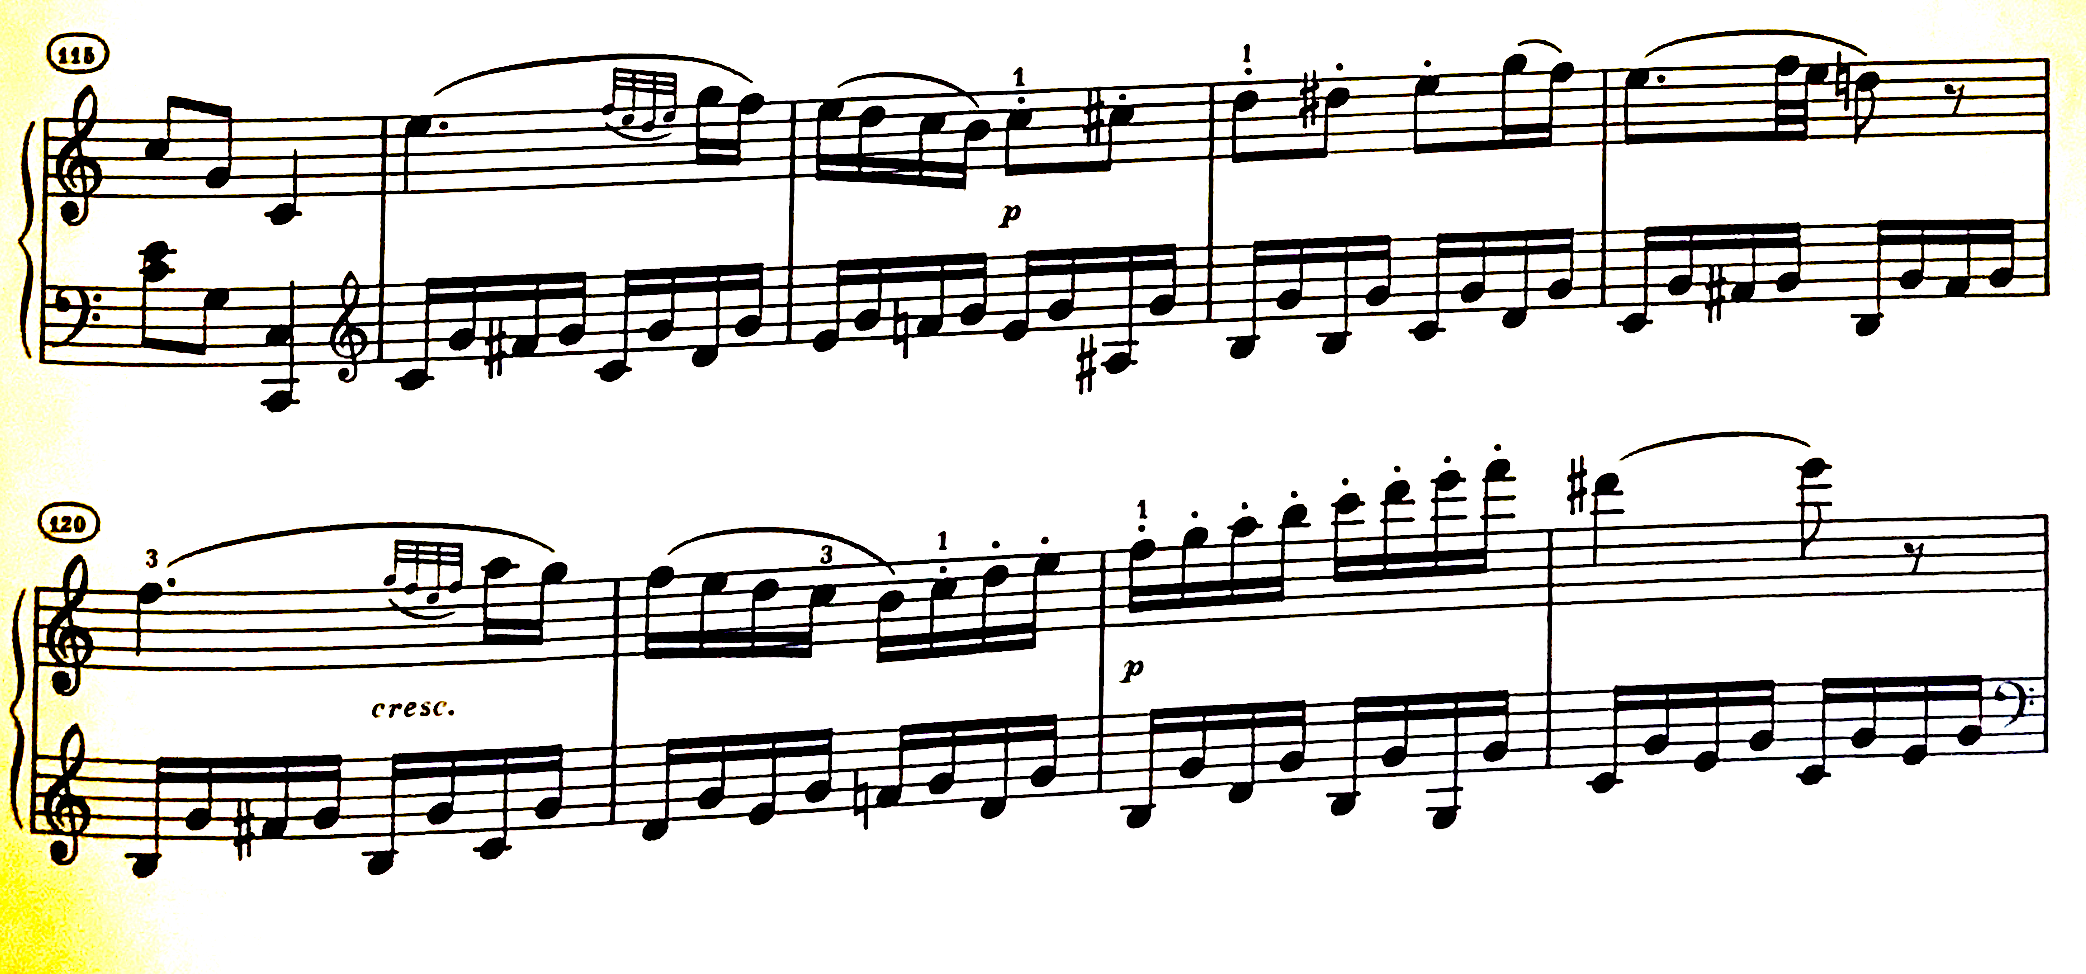
\includegraphics[width=\textwidth]{figures/mozart-third-movement-bars-116-123.jpg}
	\caption{Bars 115-123 in the third movement of Mozart's \textit{Piano Sonata in C Major}}
	\label{fig:mozart-third-movement-bars-116-123}
\end{figure}

\begin{figure}
	\centering
	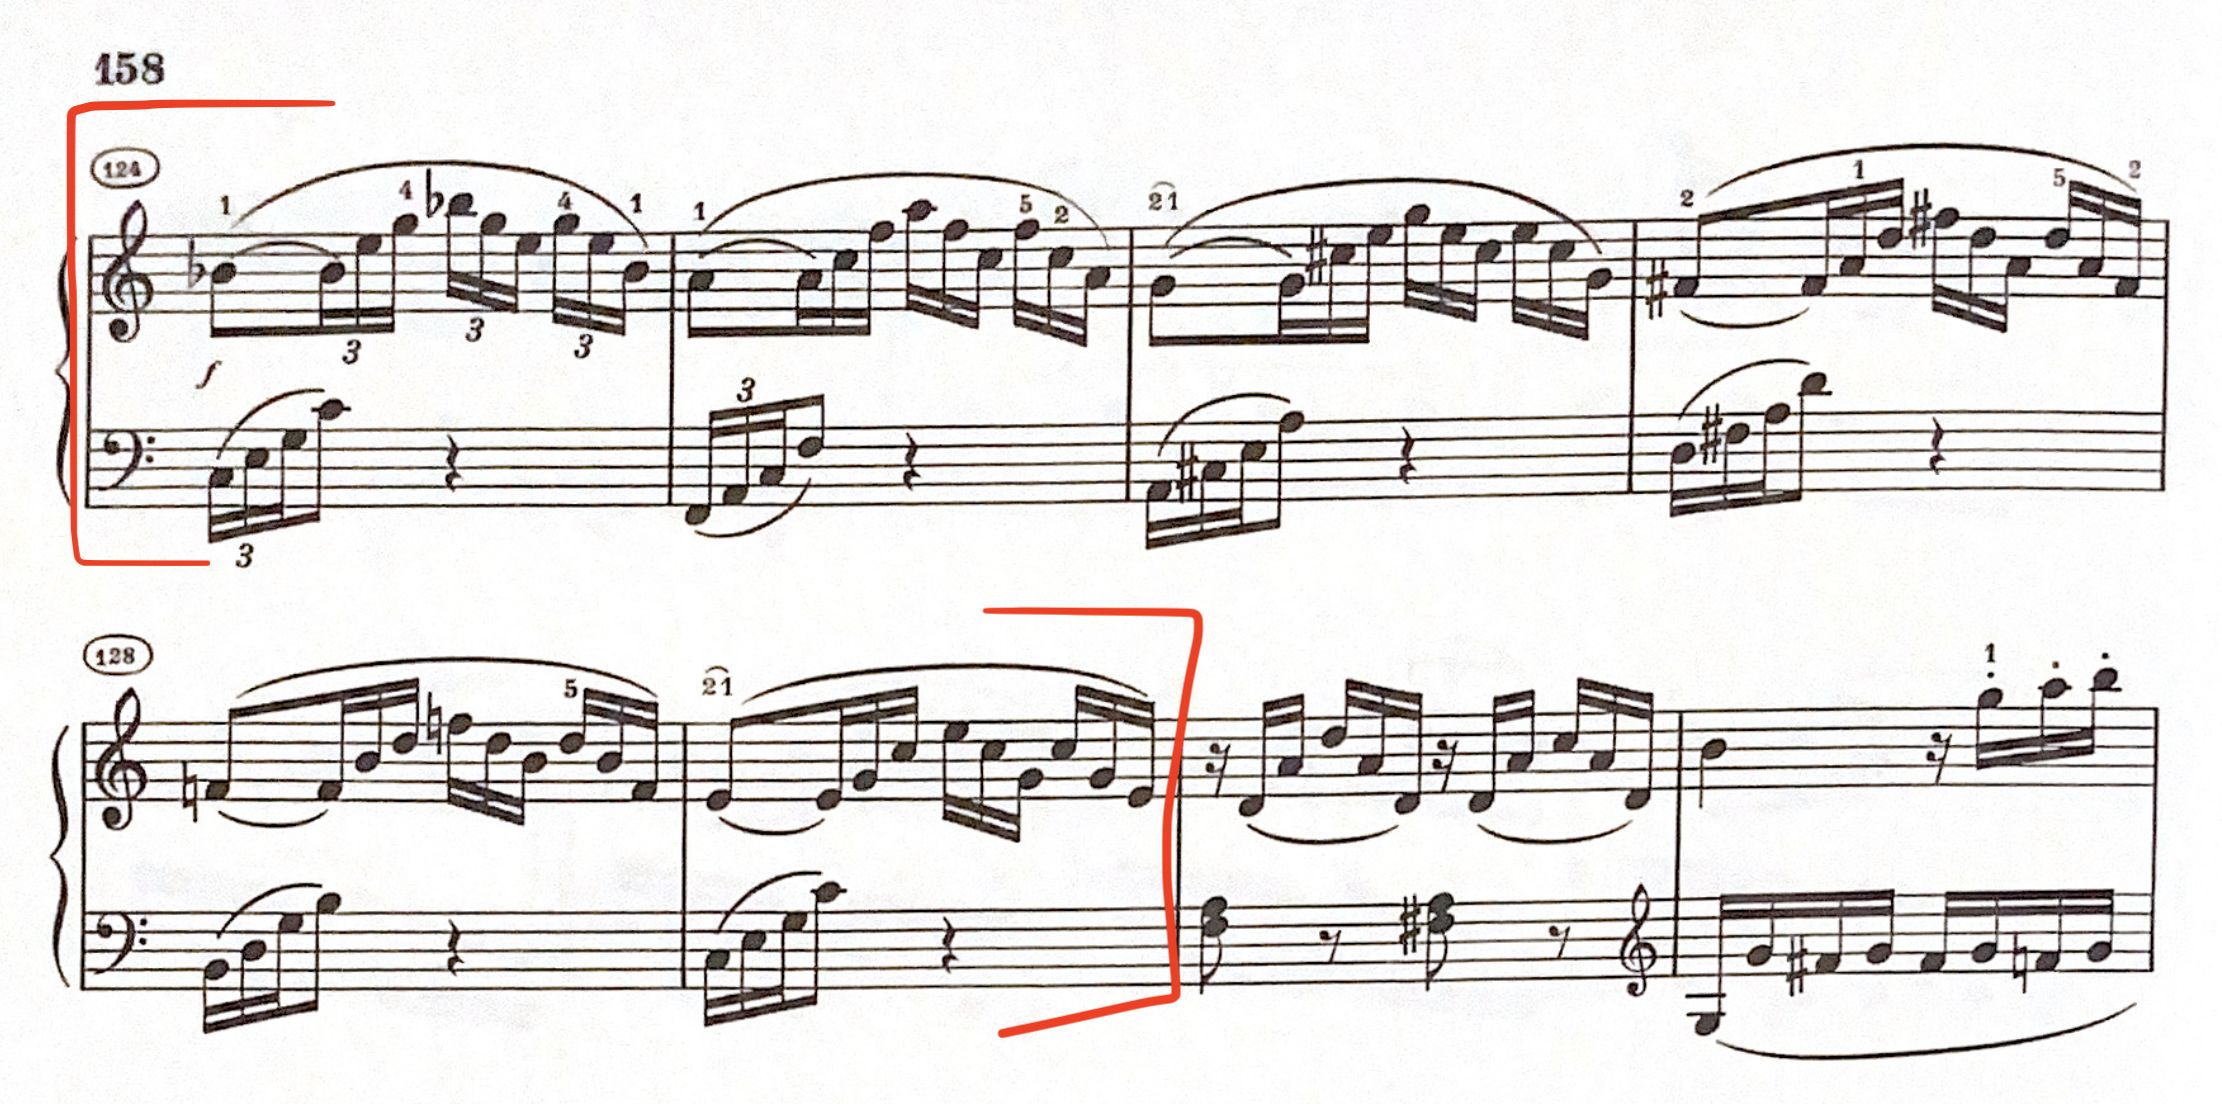
\includegraphics[width=0.5\textwidth]{figures/mozart-third-movement-bars-124-129.jpg}
	\caption{Bars 124-129 in the third movement of Mozart's \textit{Piano Sonata in C Major}}
	\label{fig:mozart-third-movement-bars-124-129}
\end{figure}

\begin{figure}
    \centering
    \includegraphics[width=\textwidth]{figures/mozart-third-movement-coda.jpg}
    \caption{Mozart's \textit{Piano Sonata in C Major}, the coda of the third movement}
    \label{fig:mozart-third-movement-coda}
\end{figure}
